\documentclass[12pt, titlepage]{article}

\usepackage{booktabs}
\usepackage{tabularx}
\usepackage{hyperref}
\usepackage{graphicx}
\usepackage{longtable}
\usepackage[utf8]{inputenc}
\usepackage[T1]{fontenc}
\usepackage{lmodern}
\usepackage{parskip}
\hypersetup{
    colorlinks,
    citecolor=black,
    filecolor=black,
    linkcolor=red,
    urlcolor=blue
}

\usepackage[round]{natbib}

%% Comments

\usepackage{color}

\newif\ifcomments\commentstrue %displays comments
%\newif\ifcomments\commentsfalse %so that comments do not display

\ifcomments
\newcommand{\authornote}[3]{\textcolor{#1}{[#3 ---#2]}}
\newcommand{\todo}[1]{\textcolor{red}{[TODO: #1]}}
\else
\newcommand{\authornote}[3]{}
\newcommand{\todo}[1]{}
\fi

\newcommand{\wss}[1]{\authornote{blue}{SS}{#1}} 
\newcommand{\plt}[1]{\authornote{magenta}{TPLT}{#1}} %For explanation of the template
\newcommand{\an}[1]{\authornote{cyan}{Author}{#1}}

%% Common Parts

\newcommand{\progname}{ProgName} % PUT YOUR PROGRAM NAME HERE
\newcommand{\authname}{Team \#, Team Name
\\ Student 1 name
\\ Student 2 name
\\ Student 3 name
\\ Student 4 name} % AUTHOR NAMES                  

\usepackage{hyperref}
    \hypersetup{colorlinks=true, linkcolor=blue, citecolor=blue, filecolor=blue,
                urlcolor=blue, unicode=false}
    \urlstyle{same}
                                


\begin{document}

\title{Verification and Validation Report: \progname} 
\author{\authname}
\date{\today}
	
\maketitle

\pagenumbering{roman}

\section{Revision History}

\begin{tabularx}{\textwidth}{p{3cm}p{2cm}X}
\toprule {\bf Date} & {\bf Version} & {\bf Notes}\\
\midrule
3/7/2025 & 1.0 & First write up of VnV Report \\
\bottomrule
\end{tabularx}

~\newpage

\section{Symbols, Abbreviations and Acronyms}

\renewcommand{\arraystretch}{1.2}
\begin{tabular}{l l} 
  \toprule		
  \textbf{symbol} & \textbf{description}\\
  \midrule 
  TPG & Tangled Program Graphs\\
  DNNs & Deep Neural Networks\\
  RL & Reinforcement Learning\\
  SRS & Software Requirement Specification\\
  FR & Functional Requirement\\
  NFR & Non-Functional Requirement\\
  SLN & System Level Number\\
  VnV & Verification and Validation\\
  \bottomrule
\end{tabular}\\

% \wss{symbols, abbreviations or acronyms -- you can reference the SRS tables if needed}

\newpage

\tableofcontents

\listoftables %if appropriate

\listoffigures %if appropriate

\newpage

\pagenumbering{arabic}

This document cohesively summarizes the results of each test as specified in the \href{https://github.com/TPGEngine/tpg/blob/main/docs/VnVPlan/VnVPlan.pdf}{VnV Plan} documentation.

\section{Functional Requirements Evaluation}

\subsection{MuJoCo Integration}\label{mujoco_integration}

\begin{center}
    \begin{longtable}{|p{2cm}|p{8cm}|p{2cm}|}
      \caption{MuJoCo Integration Tests} \\
    \hline
    \textbf{Test Id} & \textbf{Notes} & \textbf{Result} \\
    \hline
    \endfirsthead
    \hline
    \textbf{Test Id} & \textbf{Notes} & \textbf{Result} \\
    \hline
    \endhead
    FR-SLN1 & When executing the appropriate script, all MuJoCo environments can be run. The best-performing agent within the policy can be visualized using OpenGL or an MP4 file. & Pass \\
    \hline
    FR-SLN2 & MuJoCo environments within the TPG framework can be successfully run within the Digital Research Alliance, enabling research to be conducted by executing experiments. & Pass \\
    \hline
    \end{longtable}
\end{center}

\subsection{Experiment Visualization}\label{experiment_visualization}

\begin{center}
  \begin{longtable}{|p{2cm}|p{8cm}|p{2cm}|}
    \caption{Experiment Visualization Tests} \\
  \hline
  \textbf{Test Id} & \textbf{Notes} & \textbf{Result} \\
  \hline
  \endfirsthead
  \hline
  \textbf{Test Id} & \textbf{Notes} & \textbf{Result} \\
  \hline
  \endhead
  FR-SLN3 & When an experiment is running or finished training, the best performing policy can be visualized using the TPG CLI tool. & Pass \\
  \hline
  \end{longtable}
\end{center}

\pagebreak 

\subsection{Github Actions CI/CD Pipeline}\label{github_actions}

\begin{center}
  \begin{longtable}{|p{2cm}|p{8cm}|p{2cm}|}
    \caption{Github Actions CI/CD Pipeline Tests} \\
      \hline
  \textbf{Test Id} & \textbf{Notes} & \textbf{Result} \\
  \hline
  \endfirsthead
  \hline
  \textbf{Test Id} & \textbf{Notes} & \textbf{Result} \\
  \hline
  \endhead
      FR-SLN4 & Affirmed that the “Build TPG Project” pipeline properly builds the TPG framework with updated code when changes are pushed to any branch. & Pass \\
  \hline
  FR-SLN5 & When the project building pipeline runs properly, the TPG unit test cases are also automatically ran, and the build will only pass if all the unit tests passes
  . & Pass \\
  \hline

  FR-SLN6 & Tested that linting and Latex compilation pipeline works as expected. & Pass \\

  \hline
  \end{longtable}
\end{center}

\subsection{Software Engineering Practices}\label{software_engineering_practices}

\begin{center}
  \begin{longtable}{|p{2cm}|p{8cm}|p{2cm}|}
    \caption{Software Engineering Practices Tests} \\
  \hline
  \textbf{Test Id} & \textbf{Notes} & \textbf{Result} \\
  \hline
  \endfirsthead
  \hline
  \textbf{Test Id} & \textbf{Notes} & \textbf{Result} \\
  \hline
  \endhead
  FR-SLN7 & Newly added code in the TPG codebase follows Google's C++ Style Guide and software engineering best practices such as design patterns, and object-oriented design. This includes careful review and consideration of code readability, extendability, maintainability and scalability. A linter has also been implemented to check for such styling as discussed in \ref{github_actions}. & Pass \\
  \hline
  \end{longtable}
\end{center}

\section{Nonfunctional Requirements Evaluation}

\subsection{Usability}\label{usability}
		
\subsection{Performance}\label{performance}

\begin{center}
  \begin{longtable}{|p{4cm}|p{4cm}|}
  \caption{Performance Tests} \\
  \hline
  \textbf{Test Id} & \textbf{Result} \\
  \hline
  \endfirsthead
  \hline
  \textbf{Test Id} & \textbf{Result} \\
  \hline
  \endhead
  NFR-SLR4 & Pass \\
  \hline
  \end{longtable}
\end{center}

For NFR-SLN4, test cases within TPG for the experimental environments have been implemented to check for the accuracy of the numerical computations associated during training. Declaration of variables with proper types (e.g. signed long or int, unsigned long or int) has also been taken into consideration to reduce issues in the future for extremely large or small numbers that may overflow. TPG has been comprehensively tested to guarantee that all computations with high numerical precision (e.g. during the runtime of an experiment) are accurate and contain an acceptable tolerance limit of 0.00001. The results were inspected manually by comparing the actual output to the anticipated output, and performing a calculation to check for quantitative error, and if such error meets the requirements for numerical precision.

\begin{figure}[h]
  \centering
  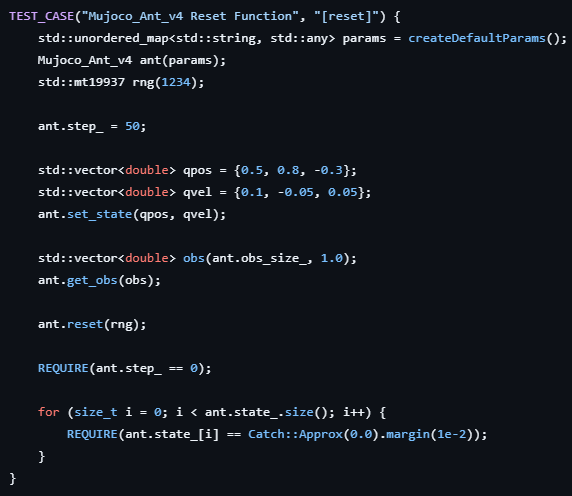
\includegraphics[width=1\textwidth]{img/ant_test.png}
  \caption{Example of a Numerical Computation Test}
\end{figure}

\subsection{Operational and Environmental}\label{operational}

\begin{center}
  \begin{longtable}{|p{4cm}|p{4cm}|}
  \caption{Operational and Environmental Tests} \\
  \hline
  \textbf{Test Id} & \textbf{Result} \\
  \hline
  \endfirsthead
  \hline
  \textbf{Test Id} & \textbf{Result} \\
  \hline
  \endhead
  NFR-SLR6 & Pass \\
  \hline
  \end{longtable}
\end{center}

For NFR-SLN6, TPG now supports contributions from macOS, Windows, and Linux developers.
Previously, only Linux was supported because TPG used SCons for C++ builds and Linux-specific dependencies from \href{https://gitlab.cas.mcmaster.ca/kellys32/tpg/-/blob/main/requirements.txt}{requirements.txt}.
With VSCode Dev Containers, a Linux development environment is automatically launched for all developers, ensuring a standardized setup.
Simply follow the \href{https://gitlab.cas.mcmaster.ca/kellys32/tpg/-/wikis/home}{Wiki} instructions to download all necessary Linux dependencies and build the C++ code reliably. Onboarding on a Macbook has been reduced from 2 weeks to just 5 minutes.


\subsection{Maintainability}\label{maintainability}

  \begin{center}
  \begin{longtable}{|p{4cm}|p{4cm}|}
  \caption{Maintainability Tests} \\
  \hline
  \textbf{Test Id} & \textbf{Result} \\
  \hline
  \endfirsthead
  \hline
  \textbf{Test Id} & \textbf{Result} \\
  \hline
  \endhead
  NFR-SLR7 & Pass \\
  \hline
  \end{longtable}
\end{center}

To satisfy the testing requirements for NFR-SLR7 - establishing a secure and robust repository management system, the team has implemented checks to ensure the repository prevents unauthorized access and defective code integration. The repository where our team is working on GitHub (whereas the base TPG repository is based in Gitlab), and access is controlled through a combination of two-factor authentication (2FA), and a main branch that is protected to ensure that merge requests can only be performed after the \href{https://github.com/TPGEngine/tpg/blob/main/.github/workflows/build-project.yaml}{TPG project GitHub workflow} action pipeline has successfully completed. This pipeline validates the building and testing process, ensuring that only code that passes all checks can be merged into the main branch. Any critical build errors or warnings, create blocking pull request conversations that must be resolved before merging. There is also a specific \href{https://github.com/TPGEngine/tpg/blob/main/.github/workflows/pull-gitlab.yml}{GitHub workflow} that is used to automatically pull changes from GitLab, eliminating the need for manual merging and risk of human error. 

\subsection{Security}\label{security}

\begin{center}
  \begin{longtable}{|p{4cm}|p{4cm}|}
  \caption{Security Tests} \\
  \hline
  \textbf{Test Id} & \textbf{Result} \\
  \hline
  \endfirsthead
  \hline
  \textbf{Test Id} & \textbf{Result} \\
  \hline
  \endhead
  NFR-SLR8 & Pass \\
  \hline
  \end{longtable}
\end{center}


For NFR-SLN8, the .csv, .txt, .png and .mp4 files that are generated within Classic Control and MuJoCo experiments are ignored by Git when making commits to the public repositories in GitHub and GitLab to reduce chance of oversharing sensitive data. Currently, none of these files generate sensitive data, but to follow best practice and to keep the repository at a clean state, these are not recognized when synchronizing code to each respective repository. Additionally, the team has also manually checked all stored .csv, .txt, .png and .mp4 files along with others that may contain textual information to see if data within them are sensitive and must be kept private. 

\subsection{Compliance}\label{compliance}

\begin{center}
\begin{longtable}{|p{4cm}|p{4cm}|}
\caption{Compliance Tests} \\
\hline
\textbf{Test Id} & \textbf{Result} \\
\hline
\endfirsthead
\hline
\textbf{Test Id} & \textbf{Result} \\
\hline
\endhead
NFR-SLR9 & Pass \\
\hline
\end{longtable}
\end{center}

The modified codebase is successfully analyzed using Clang-Tidy and Clang-Format within the CI/CD pipeline. 
Code change discussions take place through pull request conversations made to the main branch. 
All errors and warnings are generated based on the C++ Style Guidelines. 
Any critical errors found during the linting process create blocking pull request conversations that must be resolved before merging into the main branch.

\begin{figure}[h]
  \centering
  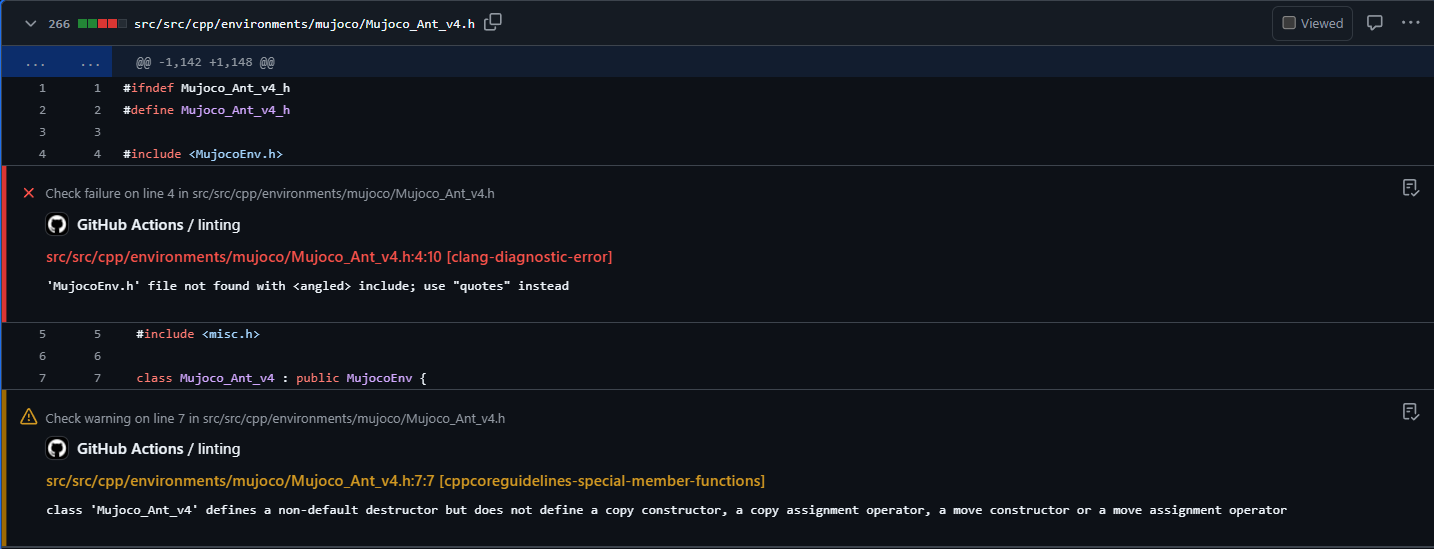
\includegraphics[width=1\textwidth]{img/linter-example.png}
  \caption{Example of a Linter Error}
\end{figure}

\section{Unit Testing}

\subsection{Behaviour-Hiding Module}

\subsubsection{RegisterMachine Crossover Tests}

\textbf{Type:} Automatic, Functional

\textbf{Initial State:} The \texttt{TPG} and \texttt{RegisterMachine} objects are initialized with default parameters and state.

\textbf{Test Case Derivation:} The expected behavior is derived from the correct crossover functionality, chunk splitting, and recombination of \texttt{RegisterMachine} objects, ensuring valid instruction patterns and segment lengths.

\textbf{Test Procedure:} The test will be performed as follows:
\begin{itemize}
    \item \textbf{Basic Crossover Functionality Test:}
    \begin{itemize}
        \item \textbf{Input:} Two parent \texttt{RegisterMachine} objects.
        \item \textbf{Output:} Two child \texttt{RegisterMachine} objects with valid instructions and actions.
        \item \textbf{Test Derivation:} Verifies that crossover produces children with reasonable sizes, valid actions, and instruction patterns derived from both parents.
    \end{itemize}

    \item \textbf{Chunk Splitting and Recombination Test:}
    \begin{itemize}
        \item \textbf{Input:} Two parent \texttt{RegisterMachine} objects with predefined instruction sequences.
        \item \textbf{Output:} Two child \texttt{RegisterMachine} objects with instruction counts and patterns derived from both parents.
        \item \textbf{Test Derivation:} Ensures that crossover produces children with valid instruction counts and different instruction patterns.
    \end{itemize}

    \item \textbf{Crossover Constraints Test:}
    \begin{itemize}
        \item \textbf{Input:} Two parent \texttt{RegisterMachine} objects with predefined instruction sequences.
        \item \textbf{Output:} Two child \texttt{RegisterMachine} objects adhering to crossover constraints.
        \item \textbf{Test Derivation:} Verifies that crossover points, segment lengths, and resulting program lengths adhere to predefined constraints (\texttt{dcmax}, \texttt{lsmax}, \texttt{dsmax}, \texttt{lmin}, \texttt{lmax}).
    \end{itemize}
\end{itemize}


\subsubsection{Team Crossover Tests}

\textbf{Type:} Automatic, Functional

\textbf{Initial State:} The \texttt{TPG} and \texttt{team} objects are initialized with default parameters and state.

\textbf{Test Case Derivation:} The expected behavior is derived from the correct crossover functionality of \texttt{team} objects, ensuring valid team sizes, atomic program preservation, and adherence to team size limits.

\textbf{Test Procedure:} The test will be performed as follows:
\begin{itemize}
    \item \textbf{Single Program Teams - Linear Crossover Test:}
    \begin{itemize}
        \item \textbf{Input:} Two parent teams with single programs.
        \item \textbf{Output:} A child team with one program.
        \item \textbf{Test Derivation:} Verifies that crossover produces a child team with a single program and valid atomic count.
    \end{itemize}

    \item \textbf{Multi-Program Teams - Team Crossover Test:}
    \begin{itemize}
        \item \textbf{Input:} Two parent teams with multiple programs.
        \item \textbf{Output:} A child team with programs derived from both parents.
        \item \textbf{Test Derivation:} Ensures that crossover produces a child team with a valid size (within \texttt{max\_team\_size}) and at least one atomic program.
    \end{itemize}

    \item \textbf{Atomic Program Preservation Test:}
    \begin{itemize}
        \item \textbf{Input:} Two parent teams with atomic and non-atomic programs.
        \item \textbf{Output:} A child team with at least one atomic program.
        \item \textbf{Test Derivation:} Verifies that crossover preserves atomic programs in the child team.
    \end{itemize}

    \item \textbf{Team Size Limits Test:}
    \begin{itemize}
        \item \textbf{Input:} Two parent teams with the maximum number of programs.
        \item \textbf{Output:} A child team with a size within \texttt{max\_team\_size}.
        \item \textbf{Test Derivation:} Ensures that crossover produces a child team adhering to the predefined team size limit.
    \end{itemize}
\end{itemize}



\subsection{Mujoco Module}

\subsubsection{Mujoco Environment Test\\}


\textbf{Type:} Automatic, Functional

\textbf{Initial State:} The MuJoCo environment is initialized using the \texttt{MockMujocoEnv} class with the appropriate model path.

\textbf{Test Case Derivation:} The expected behavior is derived from the correct initialization, state setting, and simulation execution of the MuJoCo environment.

\textbf{Test Procedure:} The test will be performed as follows:
\begin{itemize}
    \item \textbf{Simulation Initialization Test:}
    \begin{itemize}
        \item \textbf{Input:} Model path determined by the \texttt{determine\_tpg\_env()} function.
        \item \textbf{Output:} Successful initialization of the MuJoCo environment.
        \item \textbf{Test Derivation:} Verifies that the \texttt{initialize\_simulation()} function correctly initializes the MuJoCo environment, ensuring that the model (\texttt{m\_}) and data (\texttt{d\_}) pointers are not null.
    \end{itemize}

    \item \textbf{Set State Test:}
    \begin{itemize}
        \item \textbf{Input:} Position vector \texttt{qpos} set to \texttt{\{0.5, 0.5, ...\}} and velocity vector \texttt{qvel} set to \texttt{\{0.1, 0.1, ...\}}.
        \item \textbf{Output:} Updated state in the MuJoCo environment.
        \item \textbf{Test Derivation:} Ensures that the \texttt{set\_state()} function correctly updates the position and velocity states in the MuJoCo environment, verifying that \texttt{d\_->qpos} and \texttt{d\_->qvel} match the input values.
    \end{itemize}

    \item \textbf{Do Simulation Test:}
    \begin{itemize}
        \item \textbf{Input:} Control vector \texttt{control} set to \texttt{\{0.2, 0.2, ...\}} and a step count of 5.
        \item \textbf{Output:} Updated control values in the MuJoCo environment.
        \item \textbf{Test Derivation:} Confirms that the \texttt{do\_simulation()} function correctly applies the control inputs and updates the simulation state, ensuring that \texttt{d\_->ctrl} matches the input control values.
    \end{itemize}
\end{itemize}

\textbf{Test Cases}

\textbf{Test Case 1: Simulation Initialization}
\begin{itemize}
    \item \textbf{Description:} Tests the initialization of the MuJoCo simulation environment.
    \item \textbf{Steps:}
    \begin{enumerate}
        \item Create a \texttt{MockMujocoEnv} object with the model path.
        \item Call \texttt{initialize\_simulation()}.
        \item Verify that \texttt{m\_} and \texttt{d\_} are not null.
    \end{enumerate}
\end{itemize}

\textbf{Test Case 2: Set State}
\begin{itemize}
    \item \textbf{Description:} Tests the ability to set the state of the MuJoCo environment.
    \item \textbf{Steps:}
    \begin{enumerate}
        \item Create a \texttt{MockMujocoEnv} object and initialize the simulation.
        \item Set \texttt{qpos} to \texttt{\{0.5, 0.5, ...\}} and \texttt{qvel} to \texttt{\{0.1, 0.1, ...\}}.
        \item Call \texttt{set\_state(qpos, qvel)}.
        \item Verify that \texttt{d\_->qpos} and \texttt{d\_->qvel} match the input values.
    \end{enumerate}
\end{itemize}

\textbf{Test Case 3: Do Simulation}
\begin{itemize}
    \item \textbf{Description:} Tests the execution of a simulation step with control inputs.
    \item \textbf{Steps:}
    \begin{enumerate}
        \item Create a \texttt{MockMujocoEnv} object and initialize the simulation.
        \item Set \texttt{control} to \texttt{\{0.2, 0.2, ...\}}.
        \item Call \texttt{do\_simulation(control, 5)}.
        \item Verify that \texttt{d\_->ctrl} matches the input control values.
    \end{enumerate}
\end{itemize}

\subsubsection{Mujoco Ant Test\\}

\textbf{Type:} Automatic, Functional

\textbf{Initial State:} The \texttt{Mujoco\_Ant\_v4} environment is initialized.

\textbf{Test Case Derivation:} The expected value is based on the logic that the environment should be terminal when the step count reaches 200, as per the environment's design.

\textbf{Test Procedure:} The test will be performed as follows:
\begin{itemize}
    \item \textbf{Healthy Reward Test:}
    \begin{itemize}
        \item \textbf{Input:} None.
        \item \textbf{Output:} Returns \texttt{healthy\_reward\_}.
        \item \textbf{Test Derivation:} Verifies that the \texttt{healthy\_reward()} function correctly returns the predefined \texttt{healthy\_reward\_} value.
    \end{itemize}

    \item \textbf{Control Cost Test:}
    \begin{itemize}
        \item \textbf{Input:} Action vector \texttt{\{0.1, -0.1, 0.2, 0.3\}}.
        \item \textbf{Output:} Calculated control cost.
        \item \textbf{Test Derivation:} Ensures the \texttt{control\_cost()} function computes the cost using \texttt{control\_cost\_weight\_} and the squared sum of action values.
    \end{itemize}

    \item \textbf{Contact Cost Test:}
    \begin{itemize}
        \item \textbf{Input:} None.
        \item \textbf{Output:} Non-negative contact cost.
        \item \textbf{Test Derivation:} Confirms that the \texttt{contact\_cost()} function always returns a non-negative value.
    \end{itemize}

    \item \textbf{Is Healthy Test:}
    \begin{itemize}
        \item \textbf{Input:} Modify \texttt{qpos[2]} to test health conditions.
        \item \textbf{Output:} Boolean indicating health status.
        \item \textbf{Test Derivation:} Validates that \texttt{is\_healthy()} returns \texttt{true} when \texttt{qpos[2]} is within the healthy range and \texttt{false} otherwise.
    \end{itemize}

    \item \textbf{Simulation Step Test:}
    \begin{itemize}
        \item \textbf{Input:} Action vector \texttt{\{0.1, -0.1, 0.2, 0.3\}}.
        \item \textbf{Output:} Finite reward and incremented \texttt{step\_}.
        \item \textbf{Test Derivation:} Checks that \texttt{sim\_step()} processes actions correctly, updating the environment state and returning a valid reward.
    \end{itemize}

    \item \textbf{Get Observation Test:}
    \begin{itemize}
        \item \textbf{Input:} None.
        \item \textbf{Output:} Non-zero observation vector.
        \item \textbf{Test Derivation:} Ensures \texttt{get\_obs()} reflects the current state of the environment in the observation vector.
    \end{itemize}

    \item \textbf{Reset Function Test:}
    \begin{itemize}
        \item \textbf{Input:} Random number generator.
        \item \textbf{Output:} Reinitialized environment state.
        \item \textbf{Test Derivation:} Verifies that \texttt{reset()} brings the environment back to its initial state, setting \texttt{step\_} to 0 and state values close to zero.
    \end{itemize}
\end{itemize}




\subsubsection{Mujoco Half Cheetah Test\\}

\textbf{Type:} Automatic, Functional

\textbf{Initial State:} The \texttt{Mujoco\_Half\_Cheetah\_v4} environment is initialized with default parameters.

\textbf{Test Case Derivation:} The expected behavior is derived from the correct initialization, terminal condition, control cost calculation, simulation step execution, and reset functionality of the environment.

\textbf{Test Procedure:} The test will be performed as follows:
\begin{itemize}
    \item \textbf{Initialization Test:}
    \begin{itemize}
        \item \textbf{Input:} Default parameters.
        \item \textbf{Output:} Correct initialization of environment variables.
        \item \textbf{Test Derivation:} Verifies that \texttt{n\_eval\_train\_}, \texttt{n\_eval\_validation\_}, \texttt{n\_eval\_test\_}, and \texttt{max\_step\_} are set correctly.
    \end{itemize}

    \item \textbf{Terminal Condition Test:}
    \begin{itemize}
        \item \textbf{Input:} Step count set to 200.
        \item \textbf{Output:} \texttt{terminal()} returns \texttt{true}.
        \item \textbf{Test Derivation:} Ensures the environment terminates when the step count reaches 200.
    \end{itemize}

    \item \textbf{Control Cost Test:}
    \begin{itemize}
        \item \textbf{Input:} Action vector \texttt{\{0.1, -0.1, 0.2\}}.
        \item \textbf{Output:} Calculated control cost.
        \item \textbf{Test Derivation:} Confirms that \texttt{control\_cost()} computes the cost using the squared sum of action values.
    \end{itemize}

    \item \textbf{Simulation Step Test:}
    \begin{itemize}
        \item \textbf{Input:} Action vector \texttt{\{0.1, -0.1, 0.2\}}.
        \item \textbf{Output:} Finite reward and incremented step count.
        \item \textbf{Test Derivation:} Verifies that \texttt{sim\_step()} processes actions correctly and updates the step count.
    \end{itemize}

    \item \textbf{Reset Function Test:}
    \begin{itemize}
        \item \textbf{Input:} Random number generator and modified state.
        \item \textbf{Output:} Reinitialized environment state.
        \item \textbf{Test Derivation:} Ensures \texttt{reset()} resets the step count and state values to initial conditions.
    \end{itemize}
\end{itemize}


\subsubsection{Mujoco Hopper Test\\}

\textbf{Type:} Automatic, Functional

\textbf{Initial State:} The \texttt{Mujoco\_Hopper\_v4} environment is initialized with default parameters.

\textbf{Test Case Derivation:} The expected behavior is derived from the correct initialization, terminal condition, healthy reward, control cost calculation, health check, simulation step execution, observation retrieval, and reset functionality of the environment.

\textbf{Test Procedure:} The test will be performed as follows:
\begin{itemize}
    \item \textbf{Initialization Test:} Similar to Half Cheetah or Ant test, but the input is default parameters.
    
    \item \textbf{Terminal Condition Test:} Similar to Half Cheetah or Ant test, but the input includes modifying \texttt{qpos[1]} to test the healthy z range and step count.
    
    \item \textbf{Healthy Reward Test:} Similar to Half Cheetah or Ant test, but the input is none, and the output is \texttt{healthy\_reward\_}.
    
    \item \textbf{Control Cost Test:} Similar to Half Cheetah or Ant test, but the input is action vector \texttt{\{0.1, -0.1, 0.2\}}.
    
    \item \textbf{Is Healthy Test:} Similar to Half Cheetah or Ant test, but the input includes modifying \texttt{qpos[1]} and \texttt{qpos[2]} to test the healthy z range and angle range.
    
    \item \textbf{Simulation Step Test:} Similar to Half Cheetah or Ant test, but the input is action vector \texttt{\{0.1, -0.1, 0.2\}}.
    
    \item \textbf{Get Observation Test:} Similar to Half Cheetah or Ant test, but the input includes manually setting \texttt{qpos} and \texttt{qvel} to non-zero values.
    
    \item \textbf{Reset Function Test:} Similar to Half Cheetah or Ant test, but the input includes modifying \texttt{qpos}, \texttt{qvel}, and step count before resetting.
\end{itemize}

\subsubsection{Mujoco Humanoid Standup Test\\}

\textbf{Type:} Automatic, Functional

\textbf{Initial State:} The \texttt{Mujoco\_Humanoid\_Standup\_v4} environment is initialized with default parameters.

\textbf{Test Case Derivation:} The expected behavior is derived from the correct initialization, terminal condition, simulation step execution, observation retrieval, and reset functionality of the environment.

\textbf{Test Procedure:} The test will be performed as follows:
\begin{itemize}
    \item \textbf{Initialization Test:} Similar to Hopper or Half Cheetah test, but the input is default parameters.
    
    \item \textbf{Terminal Condition Test:} Similar to Hopper or Half Cheetah test, but the input is step count set to 200.
    
    \item \textbf{Simulation Step Test:} Similar to Hopper or Half Cheetah test, but the input is action vector \texttt{\{0.1, -0.1, 0.2\}}.
    
    \item \textbf{Get Observation Test:} Similar to Hopper or Half Cheetah test, but the input includes verifying non-zero observation values.
    
    \item \textbf{Reset Function Test:} Similar to Hopper or Half Cheetah test, but the input includes modifying \texttt{qpos}, \texttt{qvel}, and step count before resetting.
\end{itemize}


\subsubsection{Mujoco Inverted Double Pendulum Test\\}

\textbf{Type:} Automatic, Functional

\textbf{Initial State:} The \texttt{Mujoco\_Inverted\_Double\_Pendulum\_v4} environment is initialized with default parameters.

\textbf{Test Case Derivation:} The expected behavior is derived from the correct initialization, terminal condition, simulation step execution, observation retrieval, and reset functionality of the environment.

\textbf{Test Procedure:} The test will be performed as follows:
\begin{itemize}
    \item \textbf{Initialization Test:} Similar to Humanoid Standup or Hopper test, but the input is default parameters.
    
    \item \textbf{Terminal Condition Test:} Similar to Humanoid Standup or Hopper test, but the input includes modifying \texttt{site\_xpos[2]} to test the terminal threshold and step count.
    
    \item \textbf{Simulation Step Test:} Similar to Humanoid Standup or Hopper test, but the input is action vector \texttt{\{0.1\}}.
    
    \item \textbf{Get Observation Test:} Similar to Humanoid Standup or Hopper test, but the input includes manually setting \texttt{qpos} and \texttt{qvel} to non-zero values.
    
    \item \textbf{Reset Function Test:} Similar to Humanoid Standup or Hopper test, but the input includes modifying \texttt{qpos}, \texttt{qvel}, and step count before resetting.
\end{itemize}


\subsubsection{Mujoco Inverted Pendulum Test\\}

\textbf{Type:} Automatic, Functional

\textbf{Initial State:} The \texttt{Mujoco\_Inverted\_Pendulum\_v4} environment is initialized with default parameters.

\textbf{Test Case Derivation:} The expected behavior is derived from the correct initialization, terminal condition, simulation step execution, observation retrieval, and reset functionality of the environment.

\textbf{Test Procedure:} The test will be performed as follows:
\begin{itemize}
    \item \textbf{Initialization Test:} Similar to Inverted Double Pendulum or Humanoid Standup test, but the input is default parameters.
    
    \item \textbf{Terminal Condition Test:} Similar to Inverted Double Pendulum or Humanoid Standup test, but the input includes modifying \texttt{qpos[1]} to test the terminal threshold and step count.
    
    \item \textbf{Simulation Step Test:} Similar to Inverted Double Pendulum or Humanoid Standup test, but the input is action vector \texttt{\{0.1\}} and the expected reward is \texttt{1.0}.
    
    \item \textbf{Get Observation Test:} Similar to Inverted Double Pendulum or Humanoid Standup test, but the input includes manually setting \texttt{qpos} and \texttt{qvel} to non-zero values and verifying the observation vector.
    
    \item \textbf{Reset Function Test:} Similar to Inverted Double Pendulum or Humanoid Standup test, but the input includes modifying \texttt{qpos}, \texttt{qvel}, and step count before resetting.
\end{itemize}


\subsubsection{Mujoco Reacher Test\\}

\textbf{Type:} Automatic, Functional

\textbf{Initial State:} The \texttt{Mujoco\_Reacher\_v4} environment is initialized with default parameters.

\textbf{Test Case Derivation:} The expected behavior is derived from the correct initialization, terminal condition, control cost calculation, distance retrieval, simulation step execution, observation retrieval, and reset functionality of the environment.

\textbf{Test Procedure:} The test will be performed as follows:
\begin{itemize}
    \item \textbf{Initialization Test:} Similar to Inverted Pendulum or Inverted Double Pendulum test, but the input is default parameters.
    
    \item \textbf{Terminal Condition Test:} Similar to Inverted Pendulum or Inverted Double Pendulum test, but the input is step count set to 200.
    
    \item \textbf{Control Cost Test:} Similar to Hopper or Half Cheetah test, but the input is action vector \texttt{\{0.1, -0.1\}}.
    
    \item \textbf{Get Distance Test:} Unique to Reacher, the input is none, and the output is a distance vector of size 2.
    
    \item \textbf{Simulation Step Test:} Similar to Inverted Pendulum or Inverted Double Pendulum test, but the input is action vector \texttt{\{0.1, -0.1\}}.
    
    \item \textbf{Get Observation Test:} Similar to Inverted Pendulum or Inverted Double Pendulum test, but the input includes verifying non-zero observation values.
    
    \item \textbf{Reset Function Test:} Similar to Inverted Pendulum or Inverted Double Pendulum test, but the input includes modifying \texttt{qpos}, \texttt{qvel}, and step count before resetting.
\end{itemize}


\section{Changes Due to Testing}

% \wss{This section should highlight how feedback from the users and from 
% the supervisor (when one exists) shaped the final product.  In particular 
% the feedback from the Rev 0 demo to the supervisor (or to potential users) 
% should be highlighted.}
\subsection{Feedback from Rev 0}
The feedback given by the instructor and teaching assistant during Revision 0 was essential in guiding the next steps as the team looks toward the final demonstration.
Emphasis was placed on ensuring that usability testing was executed systematically rather than in the more ad-hoc manner initially planned by the team.
Some additional changes to be made include ensuring that unit testing and benchmarking of the implemented environments are cohesively executed and investigating whether the integration of deployment within the DRA is possible.

\section{Automated Testing}

As a result of the team’s conversion from building the project using SCons to CMake, automated testing became significantly easier to execute and debug.
To run any automated tests within a developer’s local environment, a developer can simply execute a command to build the project. 
This not only compiles everything but also runs all automated tests. If a developer wishes to run only the tests, they must navigate to the directory where the tests were already compiled (typically \texttt{/build/tests}). 
From there, the command \texttt{ctest} can be entered into the command prompt. Similar to the compilation process, all automated tests are executed once this command is run.\\

From the repository’s point of view, tests are executed using GitHub Actions or GitLab CI (depending on which repository is being viewed). 
Both linting and compilation are performed using the same commands that would be executed within a developer’s local environment. These tests run when a new pull request is made to the main branch, ensuring that all tests pass before merging.
The compiler workflow is also executed after merging into the main branch to ensure no errors or unintended changes in code behaviour have occurred. If any test or workflow fails, the logs of the workflow can be reviewed, providing a detailed summary of the reason for failure. 
This not only allows for easier debugging but also resolves the “works on my machine” issue.
		
\section{Trace to Requirements}
Please refer to the \href{https://github.com/TPGEngine/tpg/blob/main/docs/SRS/SRS.pdf}{SRS documentaion} \citep{SRS} for detailed information of each requirement.
\begin{longtable}{|p{0.45\linewidth}|p{0.45\linewidth}|}
\hline
\textbf{Req. ID} & \textbf{System Test ID} \\
\hline
FR-1 & \hyperref[mujoco_integration]{FR-SLN1}, \hyperref[mujoco_integration]{FR-SLN2} \\
\hline
FR-2 & \hyperref[experiment_visualization]{FR-SLN3} \\
\hline
FR-3 & \hyperref[github_actions]{FR-SLN4} \\
\hline
FR-4 & \hyperref[github_actions]{FR-SLN4} \\
\hline
FR-5 & \hyperref[github_actions]{FR-SLN4} \\
\hline
FR-6 & \hyperref[software_engineering_practices]{FR-SLN5} \\
\hline
FR-7 & \hyperref[github_actions]{FR-SLN4} \\
\hline
FR-8 & \hyperref[mujoco_integration]{FR-SLN2} \\
\hline
UH-E1 & \hyperref[usability]{NFR-SLN1} \\
\hline
UH-E2 & \hyperref[usability]{NFR-SLN2} \\
\hline
UH-PI1 & \hyperref[usability]{NFR-SLN3} \\
\hline
UH-L1 & \hyperref[usability]{NFR-SLN1} \\
\hline
UH-L2 & \hyperref[usability]{NFR-SLN1} \\
\hline
UH-UP1 & \hyperref[usability]{NFR-SLN1} \\
\hline
UH-UP2 & \hyperref[usability]{NFR-SLN1} \\
\hline
UH-A1 & \hyperref[usability]{NFR-SLN1} \\
\hline
PR-PA & \hyperref[performance]{NFR-SLN4} \\
\hline
OE-EPE & \hyperref[operational]{NFR-SLN6} \\
\hline
OE-OSR & \hyperref[usability]{NFR-SLN1} \\
\hline
MS-M2 & \hyperref[usability]{NFR-SLN1} \\
\hline
MS-S1 & \hyperref[usability]{NFR-SLN1}, \hyperref[maintainability]{NFR-SLN7} \\
\hline
MS-S2 & \hyperref[operational]{NFR-SLN6} \\
\hline
MS-A2 & \hyperref[operational]{NFR-SLN6} \\
\hline
SR-A1 & \hyperref[maintainability]{NFR-SLN7} \\
\hline
SR-A2 & \hyperref[maintainability]{NFR-SLN7} \\
\hline
SR-I1 & \hyperref[maintainability]{NFR-SLN7} \\
\hline
SR-P1 & \hyperref[maintainability]{NFR-SLN7}, \hyperref[security]{NFR-SLN8} \\
\hline
SR-AU1 & \hyperref[usability]{NFR-SLN2} \\
\hline
\end{longtable}
		
\section{Trace to Modules}		

\section{Code Coverage Metrics}

\bibliographystyle{plainnat}
\bibliography{../../refs/References}

\newpage{}
\section*{Appendix --- Reflection}

The information in this section will be used to evaluate the team members on the
graduate attribute of Reflection.

The purpose of reflection questions is to give you a chance to assess your own
learning and that of your group as a whole, and to find ways to improve in the
future. Reflection is an important part of the learning process.  Reflection is
also an essential component of a successful software development process.  

Reflections are most interesting and useful when they're honest, even if the
stories they tell are imperfect. You will be marked based on your depth of
thought and analysis, and not based on the content of the reflections
themselves. Thus, for full marks we encourage you to answer openly and honestly
and to avoid simply writing ``what you think the evaluator wants to hear.''

Please answer the following questions.  Some questions can be answered on the
team level, but where appropriate, each team member should write their own
response:


\begin{enumerate}
  \item What went well while writing this deliverable? 

  One part that went well for this deliverable is that valuating the functional and non functional requirements was relatively simple, as we were able to trace it back to our VNV plan and SRS report.
  \item What pain points did you experience during this deliverable, and how
    did you resolve them?
  \item Which parts of this document stemmed from speaking to your client(s) or
  a proxy (e.g. your peers)? Which ones were not, and why?
  \item In what ways was the Verification and Validation (VnV) Plan different
  from the activities that were actually conducted for VnV?  If there were
  differences, what changes required the modification in the plan?  Why did
  these changes occur?  Would you be able to anticipate these changes in future
  projects?  If there weren't any differences, how was your team able to clearly
  predict a feasible amount of effort and the right tasks needed to build the
  evidence that demonstrates the required quality?  (It is expected that most
  teams will have had to deviate from their original VnV Plan.)
\end{enumerate}

\end{document}